\begin{frame}{Numerical Simulation: Acquisition Design}
	\uncover<1>{%
		\begin{itemize}
			\item{Simulated many WM-like, GM-like voxel realizations}
			\item{Studied sample statistics of $\To,\Tt$ ML estimates $\ToML,\TtML$}
		\end{itemize}
	}
	\uncover<1>{%
  	\begin{table} [!tb]
      \centering
      {\tabulinesep = 0.2mm
      \begin{tabu} {c | r r r | r}
          \hline \hline
          Profile     & $(2,1)$           & $(1,1)$           & $(0,2)$           & Truth \\
          \hline
          WM $\ToML$  & $830 \pm 17$      & $830 \pm 15$      & $830 \pm 14$      & $832$ \\
          GM $\ToML$  & $1330 \pm 30.$    & $1330 \pm 24$     & $1330 \pm 24$     & $1331$ \\
          \hline
          WM $\TtML$  & $80. \pm 1.0$     & $80. \pm 2.1$     & $79.6 \pm 0.94$   & $79.6$ \\
          GM $\TtML$  & $110. \pm 1.4$    & $110. \pm 3.0$    & $110. \pm 1.6$    & $110$ \\
          \hline \hline
      \end{tabu}}
      \caption{$\ToML,\TtML$ sample means $\pm$ sample standard deviations}
      \label{table:numerical}
  	\end{table}
	}
\end{frame}

\begin{frame}{A Function Space over which Optimization is Tractable}
	\uncover<1>{%
		\textbf{Hilbert space}: complete inner product function space
		\vspace{0.5cm}
	}
	\uncover<1->{%
  	\hlb{\textbf{Reproducing kernel Hilbert space (RKHS)}} \\
  	Hilbert space $\hlb{\hilb}$ over input space $\setQ$ with \emph{reproducing property}
  	$$\innprod{h}{\hlm{k}(\cdot,\bmq)}_{\hlb{\hilb}} = h(\bmq), 
  		\qquad \forall h \in \hlb{\hilb}, \bmq \in \setQ$$ 
  	for some $\hlm{k} : \setQ^2 \mapsto \real$ called a \hlm{reproducing kernel (RK)} \\
  	\vspace{0.5cm}
	}
  \uncover<1->{%
  	\textbf{Relevant facts}
  	\begin{itemize}
  		\item{Bijection between RKHS $\hlb{\hilb}$ and RK $\hlm{k}$ 
  			\hfill \citec{aronszajn:50:tor}}
			\item{Function $\hlm{k}(\cdot,\bmq) \in \hlb{\hilb}$ 
  			called a \emph{feature mapping}}
  	\end{itemize}
	}
\end{frame}

\begin{frame}{Function Optimization over a RKHS}
	\uncover<1>{%
		\textbf{Choose}: RK $\hlm{k} : \setQ^2 \mapsto \real$
			that induces choice of RKHS $\hlb{\hilb}$ \\
	}%
	\uncover<1>{%
		\textbf{Solve}: for each desired latent parameter $l \in \set{1,\dots,L}$,
		\begin{align}
			\paren{\est{h}_l,\est{b}_l} \in 
				\set{\argmin{\substack{h_l \in \hlb{\hilb} \\ b_l \in \real}}
				\frac{1}{N} \sum_{n=1}^N \paren{h_l\paren{\bmq_n} + b_l - x_{l,n}}^2
				+ \rho_l \norm{h_l}^2_{\hlb{\hilb}}}
			\label{eq:krr,cost}
		\end{align}
	}%
	\begin{itemize}
		\item<1>{%
			Optimal $\est{h}_l$ over $\hlb{\hilb}$ takes form \hfill \citec{scholkopf:01:agr}
			\begin{align}
				\est{h}_l\paren{\cdot} \equiv \sum_{n=1}^N \est{a}_{l,n} \hlm{k}\paren{\cdot,\bmq_{n}}
				\label{eq:gen-rep}
			\end{align}
		}%
  	\item<1>{%
  		Plug \eqref{eq:gen-rep} into \eqref{eq:krr,cost}; 
  			solve now instead for $\paren{\est{a}_l,\est{b}_l}$; construct:
  		\begin{align}
  			\est{x}_l\paren{\cdot} = 	
  				\sum_{n=1}^N \est{a}_{l,n} \hlm{k}\paren{\cdot,\bmq_n} + \est{b}_l
  			\label{eq:krr,sol}
  		\end{align}
  	}%
	\end{itemize}
\end{frame}

\begin{frame}{Numerical Simulation: PERK Estimation}
  \begin{table}[!ht]
  	\tiny
  	\centering
  	\begin{tabular}{c | r | r r r}
  		\hline
  		\hline
  								& Truth 	& VPM 													
  													& PGPM 																	& PERK \\
  		\hline
  		WM $\To$ 		& $832$ 	& \mnstd{832.1}{17.2} $(17.2)$	
  													& \mnstd{832.1}{16.2} $(16.2)$ 					& \mnstd{833.0}{16.5} $(16.5)$ \\
  		GM $\To$ 		& $1331$ 	& \mnstd{1331.5}{31.1} $(31.1)$ 
  													& \mnstd{1331.2}{29.7} $(29.7)$ 				& \mnstd{1332.1}{30.4} $(30.4)$ \\ 
  		\hline
  		WM $\Tt$ 		& $79.6$	& \mnstd{79.61}{0.988} $(0.988)$
  													& \mnstd{79.60}{0.952} $(0.952)$ 				& \mnstd{79.46}{0.978} $(0.989)$ \\
  		GM $\Tt$ 		& $110.$ 	& \mnstd{110.02}{1.40} $(1.40)$
  													& \mnstd{110.02}{1.35} $(1.35)$ 				& \mnstd{109.91}{1.35} $(1.35)$ \\
      \hline
      \hline
    \end{tabular}
    \caption{%
    	Sample means $\pm$ sample standard deviations (RMSEs)
  		of VPM, PGPM, and PERK $\mzero,\To,\Tt$ estimates,
  		computed in simulation
  		over $7810$ WM-like and $9162$ GM-like voxels.
  	}
  	\label{tab:perk,sim}
  \end{table}
\end{frame}

\begin{frame}{Mismatch in Scan Design vs. Sampling Dist Support}
	\uncover<1->{%
  	\begin{figure}
  		\centering
  		\subfloat{%
				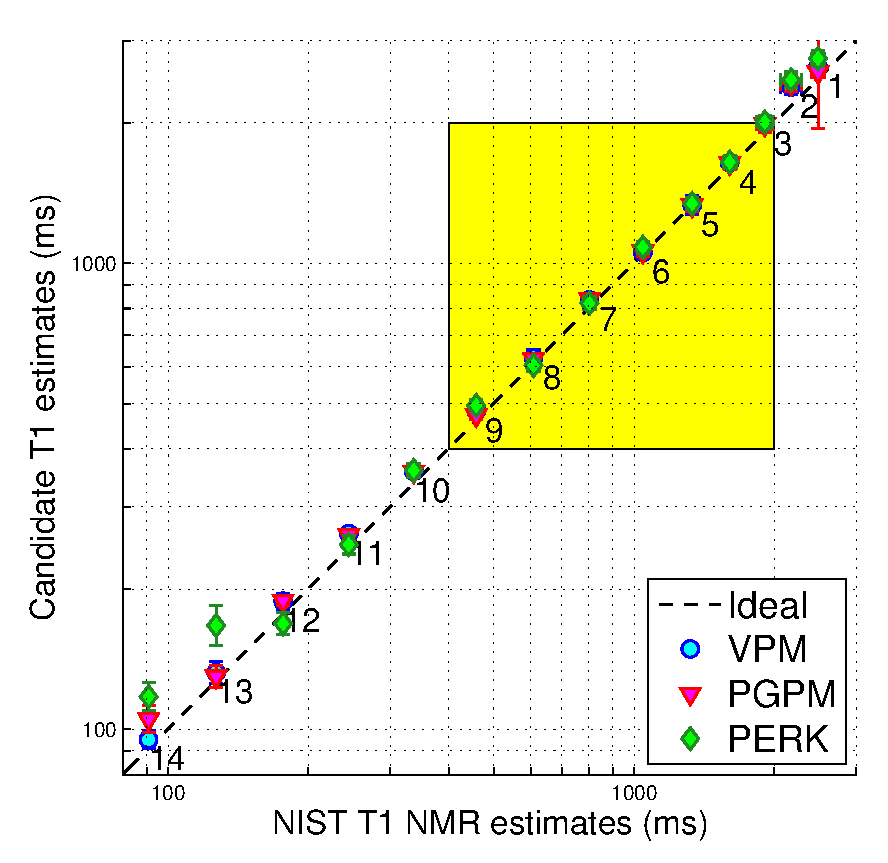
\includegraphics [width=0.45\textwidth] 
          {c,perk/hpd-broad/sp2de1,sl-6,t1,plot.eps}
        \label{fig:perk,hpd,t1}
      }%
      \hspace{0.3cm}
      \subfloat{%
      	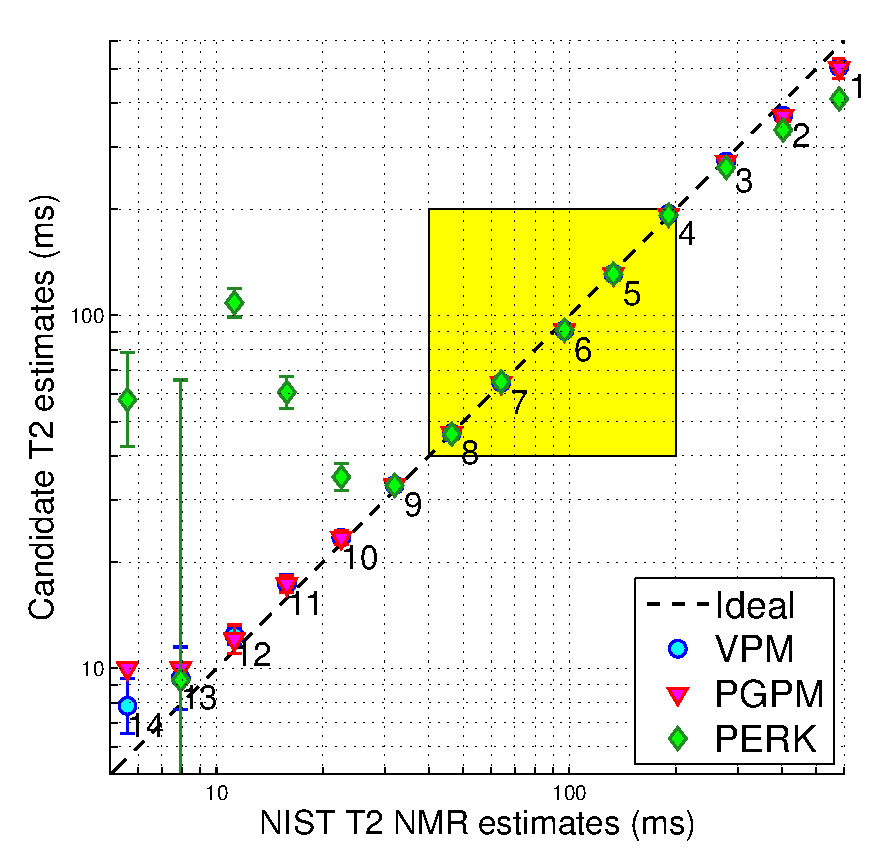
\includegraphics [width=0.45\textwidth] 
					{c,perk/hpd-broad/sp2de1,sl-6,t2,plot.eps}
				\label{fig:perk,hpd,t2}
      }%
      \label{fig:perk,hpd}
   	\end{figure}
	}%
	\uncover<1->{%
		Widening $\supp{\dist{\bmx,\bmnu}}$ degrades performance w/in scan design range.\\
		Thus, scan design and param est should be considered in tandem.
	}%
\end{frame}
